% !TEX program = xelatex
% In emacs, use this to set default compiler to xelatex:
% M-x TeX-engine-set RET xetex RET

\documentclass[xcolor=table,aspectratio=169]{beamer}

\usepackage{fancyvrb}
\usepackage{array}
\usepackage{booktabs}

\setbeamertemplate{navigation symbols}{}

\usepackage{listings}

\usepackage{graphicx}
\usepackage{hanging}
\usepackage{natbib} %citep and citet
\usepackage{amsmath}
\usepackage{mathtools}

\usepackage{xltxtra}
\setsansfont{Arial}
\setmonofont[Mapping=tex-text]{Fira Code}

\bibliographystyle{apalike}

\usetheme{Amsterdam2}
\usecolortheme{rose}
%%%%%%%%%%%%%%%%%%%%%%%%%%%%%%%%%%%%%%%%%%%

\usepackage{fancyvrb}
\newcommand{\VerbBar}{|}
\newcommand{\VERB}{\Verb[commandchars=\\\{\}]}
\DefineVerbatimEnvironment{Highlighting}{Verbatim}{commandchars=\\\{\}}
% Add ',fontsize=\small' for more characters per line
\usepackage{framed}
\definecolor{shadecolor}{RGB}{248,248,248}
\newenvironment{Shaded}{\begin{snugshade}}{\end{snugshade}}
\newcommand{\KeywordTok}[1]{\textcolor[rgb]{0.13,0.29,0.53}{\textbf{{#1}}}}
\newcommand{\DataTypeTok}[1]{\textcolor[rgb]{0.13,0.29,0.53}{{#1}}}
\newcommand{\DecValTok}[1]{\textcolor[rgb]{0.00,0.00,0.81}{{#1}}}
\newcommand{\BaseNTok}[1]{\textcolor[rgb]{0.00,0.00,0.81}{{#1}}}
\newcommand{\FloatTok}[1]{\textcolor[rgb]{0.00,0.00,0.81}{{#1}}}
\newcommand{\ConstantTok}[1]{\textcolor[rgb]{0.00,0.00,0.00}{{#1}}}
\newcommand{\CharTok}[1]{\textcolor[rgb]{0.31,0.60,0.02}{{#1}}}
\newcommand{\SpecialCharTok}[1]{\textcolor[rgb]{0.00,0.00,0.00}{{#1}}}
\newcommand{\StringTok}[1]{\textcolor[rgb]{0.31,0.60,0.02}{{#1}}}
\newcommand{\VerbatimStringTok}[1]{\textcolor[rgb]{0.31,0.60,0.02}{{#1}}}
\newcommand{\SpecialStringTok}[1]{\textcolor[rgb]{0.31,0.60,0.02}{{#1}}}
\newcommand{\ImportTok}[1]{{#1}}
\newcommand{\CommentTok}[1]{\textcolor[rgb]{0.56,0.35,0.01}{\textit{{#1}}}}
\newcommand{\DocumentationTok}[1]{\textcolor[rgb]{0.56,0.35,0.01}{\textbf{\textit{{#1}}}}}
\newcommand{\AnnotationTok}[1]{\textcolor[rgb]{0.56,0.35,0.01}{\textbf{\textit{{#1}}}}}
\newcommand{\CommentVarTok}[1]{\textcolor[rgb]{0.56,0.35,0.01}{\textbf{\textit{{#1}}}}}
\newcommand{\OtherTok}[1]{\textcolor[rgb]{0.56,0.35,0.01}{{#1}}}
\newcommand{\FunctionTok}[1]{\textcolor[rgb]{0.00,0.00,0.00}{{#1}}}
\newcommand{\VariableTok}[1]{\textcolor[rgb]{0.00,0.00,0.00}{{#1}}}
\newcommand{\ControlFlowTok}[1]{\textcolor[rgb]{0.13,0.29,0.53}{\textbf{{#1}}}}
\newcommand{\OperatorTok}[1]{\textcolor[rgb]{0.81,0.36,0.00}{\textbf{{#1}}}}
\newcommand{\BuiltInTok}[1]{{#1}}
\newcommand{\ExtensionTok}[1]{{#1}}
\newcommand{\PreprocessorTok}[1]{\textcolor[rgb]{0.56,0.35,0.01}{\textit{{#1}}}}
\newcommand{\AttributeTok}[1]{\textcolor[rgb]{0.77,0.63,0.00}{{#1}}}
\newcommand{\RegionMarkerTok}[1]{{#1}}
\newcommand{\InformationTok}[1]{\textcolor[rgb]{0.56,0.35,0.01}{\textbf{\textit{{#1}}}}}
\newcommand{\WarningTok}[1]{\textcolor[rgb]{0.56,0.35,0.01}{\textbf{\textit{{#1}}}}}
\newcommand{\AlertTok}[1]{\textcolor[rgb]{0.94,0.16,0.16}{{#1}}}
\newcommand{\ErrorTok}[1]{\textcolor[rgb]{0.64,0.00,0.00}{\textbf{{#1}}}}
\newcommand{\NormalTok}[1]{{#1}}

%%%%%%%%%%%%%%%%%%%%%%%%%%%%%%%%%%%%%%%%%%%%%
\usepackage{color}
\definecolor{mygreen}{rgb}{0,0.6,0}
\definecolor{mygray}{rgb}{0.5,0.5,0.5}
\definecolor{mymauve}{rgb}{0.58,0,0.82}
\definecolor{ForestGreen}{rgb}{0.13,0.54,0.13}

\beamersetuncovermixins{\opaqueness<1>{25}}{\opaqueness<2->{15}}


%%186     206     17      38      #CE1126        
            
\title[Supervised learning-classification (2/2)]{
	{\LARGE{Statistical learning and Visualization}:\\\large{Supervised learning - classification (2/2)}}
}
\institute{
	\footnotesize Department of Methodology and Statistics\\
}
\author[van Kesteren]{Erik-Jan van Kesteren}
\date{
\includegraphics[height=1.5cm]{pics/uu-logo.png}\\
	
	\footnotesize{\emph{Applied Data Science}}}


\newcommand{\referto}[1]{\hfill{\scriptsize{\emph{\color{gray}{#1}}}}}


\begin{document}

\begin{frame}
	\maketitle
\end{frame}

\begin{frame}
	\tableofcontents
\end{frame}

\section{Introduction}\subsection{}
%\begin{frame}
%	\begin{tabular}[h]{lll}
%		\toprule
%		& What: & When:\\
%		\midrule
%		0. &Introduction & Week 1\\
%		\\
%		1.& Exploratory Data Analysis (EDA) & Week 2\\
%		2.& Supervised learning: regression & Weeks 3 \& 4\\
%		3.& \textbf{Supervised learning: classification} & Weeks 5 \& 6\\
%		4.& TBD & Week 7\\
%		5.& Unsupervised learning & Weeks 8 \& 9\\
%		\\
%		6. & \textbf{Exam} & \textbf{05 Feb 2021} \\
%		\bottomrule
%	\end{tabular}
%\end{frame}
%\begin{frame}
%	Questions about last week
%	
%	\begin{enumerate}
%		\item We are predicting whether a person will win a Nobel prize or not. The test \textbf{accuracy} of our model is 0.99 and the \textbf{F1 score} 0.12. Why the difference?
%		
%		\item Is \textbf{calibration} important for the following applications? Why (not)?
%		\begin{enumerate}
%			\item Cardiac patients come into the hospital. Based on their lab diagnostics and echos, assign each patient a risk score;
%			\item A car collects visual and Lidar data to predict whether there is a pedestrian in front of the car;
%			%\item High schools in the Netherlands are ranked based on whether they are above or below their expected final exam score, as predicted from student body composition (``value added score''); 
%			\item You would like to build a house along the Maas river. To insure the house, the insurance company predicts the risk of flooding of the area based on the location and projected climate changes in the coming decades.
%		\end{enumerate}
%	\end{enumerate}
%\end{frame}

\begin{frame}
	{Last week}
	Any questions about last week?
	
	\begin{itemize}
		\item Classification
		\item KNN
		\item Logistic regression
		\item Linear discriminant analysis
		\item Generative vs discriminative
		\item Trees
		\item Confusion matrix
	\end{itemize}
\end{frame}

\begin{frame}
	{Important concepts today}
	
	\begin{itemize}
		\item Confusion matrix, FP, FN
		\item Sensitivity, Specificity, Accuracy, Error rate
		\item Precision, PPV, NPV
		\item F1
		\item ROC curve, AUC
		\item Calibration
		\item Bootstrap resampling
		\item Ensemble methods
		\item Bagging
		\item Random forest
		\item Boosting
	\end{itemize}
\end{frame}



\section{Evaluating classifiers}

\subsection{}

\begin{frame}{Question}
	You create a model to predict whether researchers will win a Nobel prize. The test accuracy of the model is 0.999. Is this a good model?
\end{frame}

\begin{frame}
	Evaluating classifiers
\end{frame}

\begin{frame}
	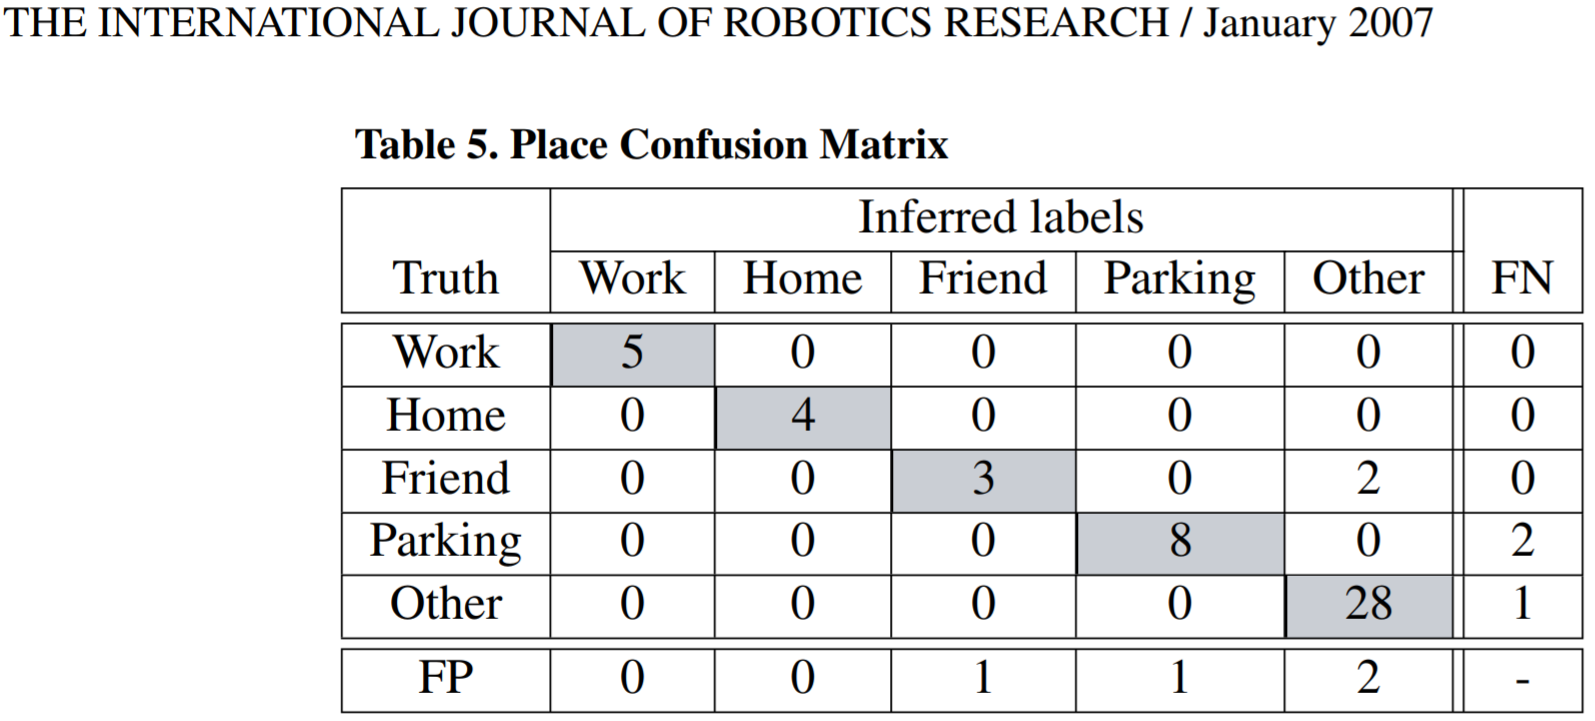
\includegraphics[width=\textwidth]{pics/confusion-place.png}
\end{frame}

\begin{frame}
	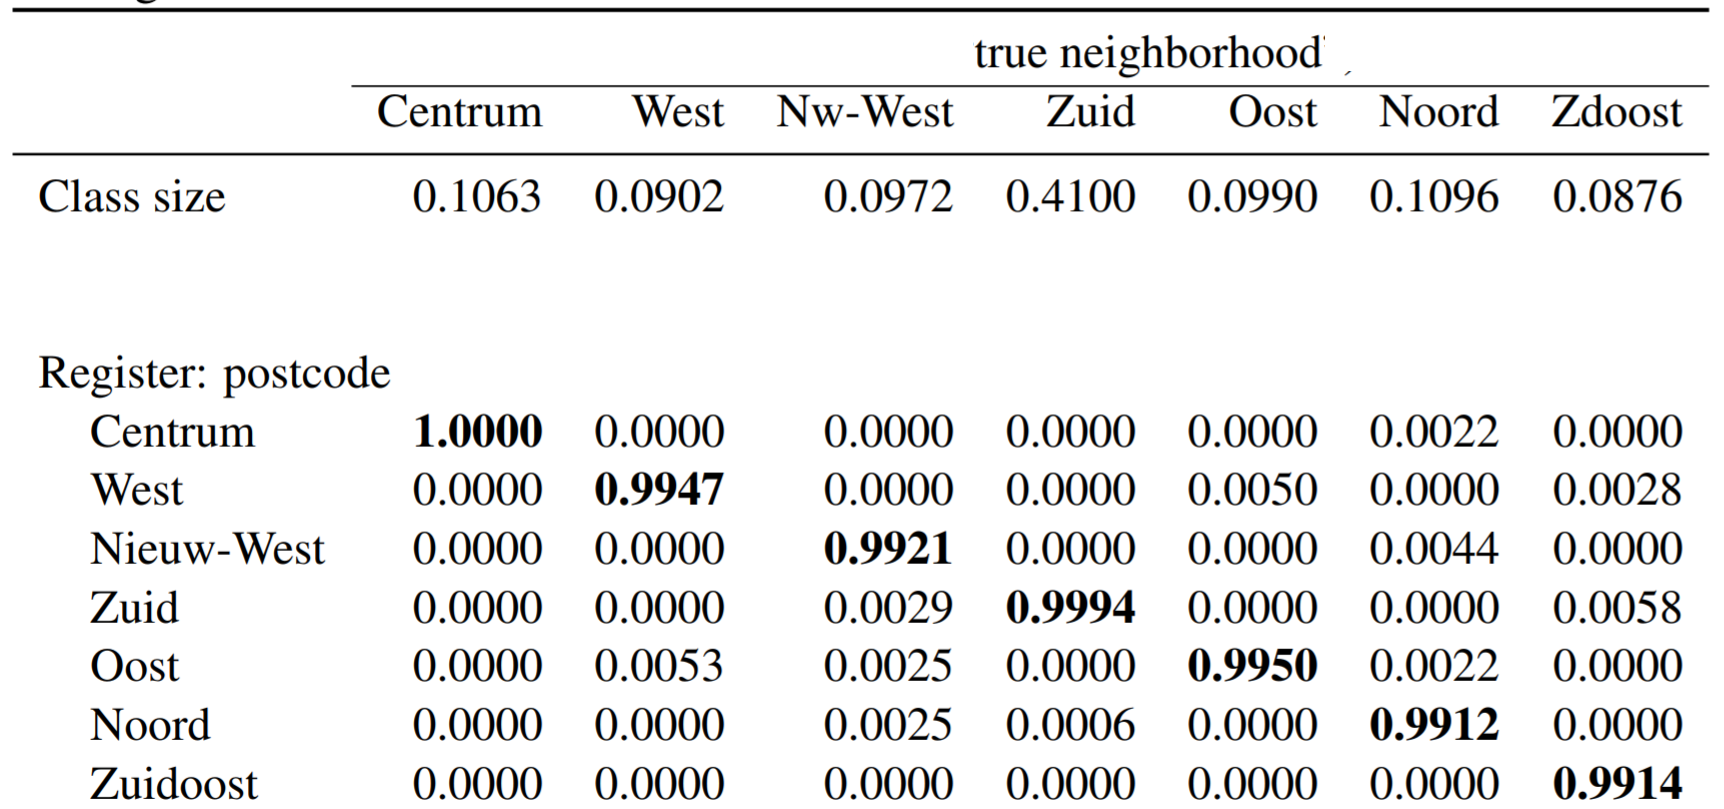
\includegraphics[width=\textwidth]{pics/LCA}
\end{frame}

\begin{frame}{Prediction tree: wood you survive the \emph{Titanic}?}
	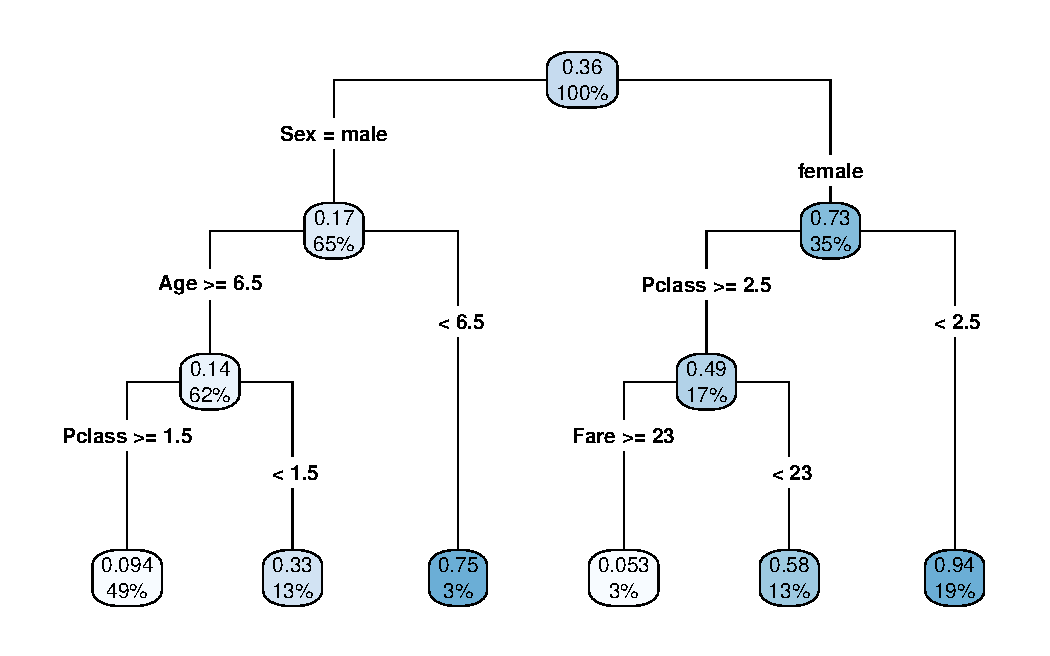
\includegraphics[width=0.78\textwidth]{pics/Titanic_tree}
\end{frame}

\begin{frame}[fragile]{Confusion matrix: Counts}
	\begin{footnotesize}
\begin{verbatim}
> p_pred <- predict(titanic_tree, newdata = val_df)

> with(val_df, table(p_pred > 0.5, Survived))

      Survived
      0   1
FALSE 134  40
TRUE   19  75
\end{verbatim}
	\end{footnotesize}
\end{frame}

\begin{frame}
	{Confusion matrix: Counts}
	
	\begin{tabular}[h]{llrrrrr}
		\toprule
		&    &\multicolumn{4}{c}{Survived (observed)}\\
		&   & No & &&Yes\\
		\midrule
		
		\multicolumn{2}{c}{Survived (predicted)}\\
		& No & \color{ForestGreen}{134} & (TN) & &  \color{red}{40} & (FN)\\
		& Yes & \color{red}{19} & (FP)& & \color{ForestGreen}{75} & (TP)\\
		\bottomrule
	\end{tabular}
	
	\bigskip
	\begin{itemize}
		\item False positives (FP): {\color{red}{19}}
		\item False negatives (FN): {\color{red}{40}}
		\item Total errors: FP + FN
	\end{itemize}
\end{frame}


\begin{frame}[fragile]
	{Confusion matrix: Sensivity (``recall'') and Specificity}
	
	\begin{scriptsize}
		\begin{verbatim}
> with(val_df, table(p_pred > 0.5, Survived)) %>% prop.table(2)
\end{verbatim}
	\end{scriptsize}\bigskip
	
	\begin{tabular}[h]{llrr}
		\toprule
		&    &\multicolumn{2}{c}{Survived (observed)}\\
		&   & No & Yes\\
		\midrule
		
		\multicolumn{2}{c}{Survived (predicted)}\\
		& No & \color{ForestGreen}{0.876} & \color{red}{0.348} \\
		& Yes & \color{red}{0.124} & \color{ForestGreen}{0.652}\\
		\midrule
		& TOTAL & 1 & 1\\
		\bottomrule
	\end{tabular}
	
	\bigskip
	\begin{itemize}
		\item Specificity: $\frac{\text{TN}}{\text{TN} + \text{FP}}$ =
		{\color{ForestGreen}{134}} / ({\color{ForestGreen}{134}} +
		{\color{red}{19}}) $\approx 0.876$
		\item Sensitivity (``recall''):
		$\frac{\text{TP}}{\text{TP} + \text{FN}}$ =
		{\color{ForestGreen}{75}} / ({\color{ForestGreen}{75}} +
		{\color{red}{40}}) $\approx 0.652$
		\item Accuracy (ACC):     $\frac{\text{TP} + \text{TN}}{\text{TP} + \text{FP} + \text{TN} + \text{FN}} \approx 0.780$
		\item Error rate: $1 - \text{Accuracy} \approx 0.220$
	\end{itemize}
\end{frame}


\begin{frame}[fragile]
	{Confusion matrix: Positive (``precision'') and Negative predictive value}
	
	\begin{scriptsize}
		\begin{verbatim}
> with(val_df, table(p_pred > 0.5, Survived)) %>% prop.table(1)
\end{verbatim}
	\end{scriptsize}\bigskip
	
	\begin{tabular}[h]{llrrr}
		\toprule
		&    &\multicolumn{2}{c}{Survived (observed)} & TOTAL\\
		&   & No & Yes\\
		\midrule
		
		\multicolumn{2}{c}{Survived (predicted)}\\
		& No & \color{ForestGreen}{0.770} & \color{red}{0.230}  & 1\\
		& Yes & \color{red}{0.202} & \color{ForestGreen}{0.798} & 1\\
		\bottomrule
	\end{tabular}
	
	\bigskip
	\begin{itemize}
		\item NPV: $\frac{\text{TN}}{\text{TN} + \text{FN}}$ =
		{\color{ForestGreen}{134}} / ({\color{ForestGreen}{134}} +
		{\color{red}{40}}) $\approx 0.770$
		\item PPV (``precision''): $\frac{\text{TP}}{\text{TP} + \text{FP}}$
		= {\color{ForestGreen}{75}} / ({\color{ForestGreen}{75}} +
		{\color{red}{19}}) $\approx 0.798$    
	\end{itemize}
\end{frame}

\begin{frame}
	{F1 score}
	The $F_1$ score is the harmonic mean of precision and recall:
	$$
	F_1 = 2 \cdot \frac{1}{\tfrac{1}{\mathrm{recall}} + \tfrac{1}{\mathrm{precision}}} = 2 \cdot \frac{\mathrm{precision} \cdot \mathrm{recall}}{\mathrm{precision} + \mathrm{recall}}
	$$
	
	\bigskip
	
	\begin{itemize}
		\item Like \textbf{accuracy}, the $F_1$ quantifies overall amount of
		error
		\item Unlike accuracy, F1 is not as affected by uneven class distributions
	\end{itemize}
\end{frame}

\begin{frame}
	{Overview}
	
	\begin{itemize}
		\item Sensitivity (=Recall)
		\item Specificity
		\item Positive predictive value (=Precision)
		\item Negative predictive value
		\item Accuracy
		\item Even more: \url{https://en.wikipedia.org/wiki/Confusion_matrix}
	\end{itemize}
\end{frame}


\begin{frame}[fragile]{Different thresholds than 0.5}
	
	\begin{scriptsize}
		\begin{verbatim}
> with(val_df, table(p_pred > 0.4, Survived)) %>% prop.table(2)

      Survived
      0     1
FALSE 0.876 0.348
TRUE  0.124 0.652

> with(val_df, table(p_pred > 0.6, Survived)) %>% prop.table(2)

      Survived
      0     1
FALSE 0.961 0.522
TRUE  0.039 0.478
\end{verbatim}
	\end{scriptsize}
	Etc.
	
	Moving around the threshold affects the sensitivity and specificity!
\end{frame}

\begin{frame}
	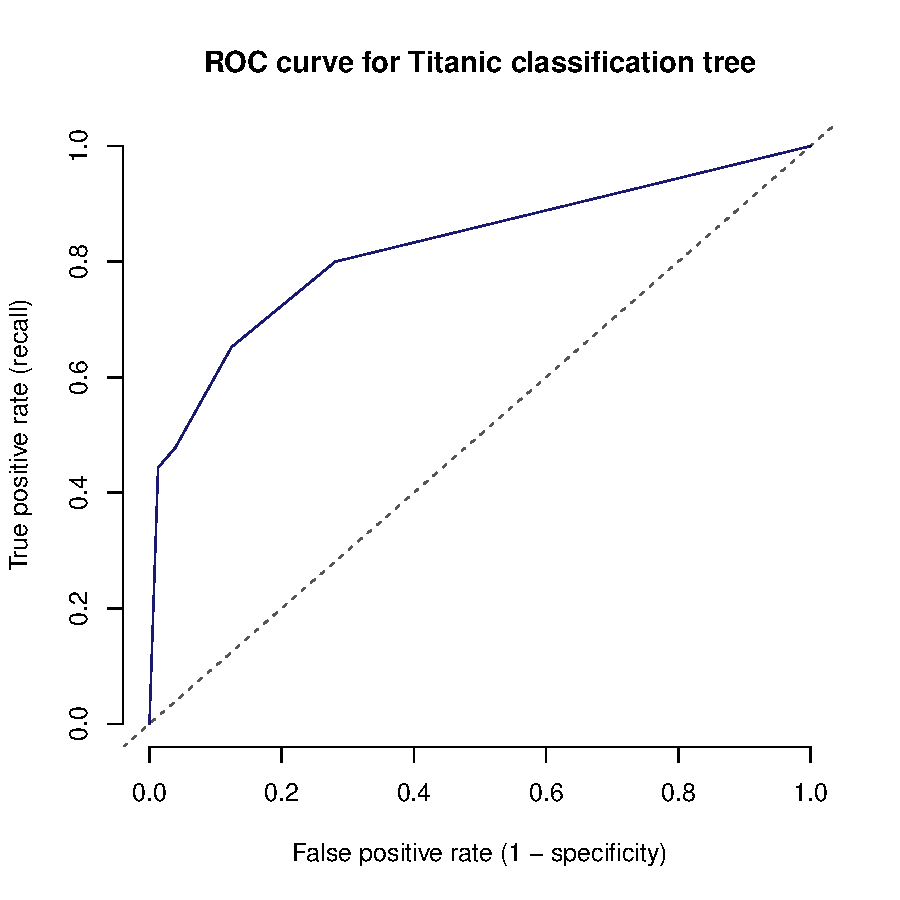
\includegraphics[height=\textheight]{pics/Titanic_tree_roc}
\end{frame}

\begin{frame}
	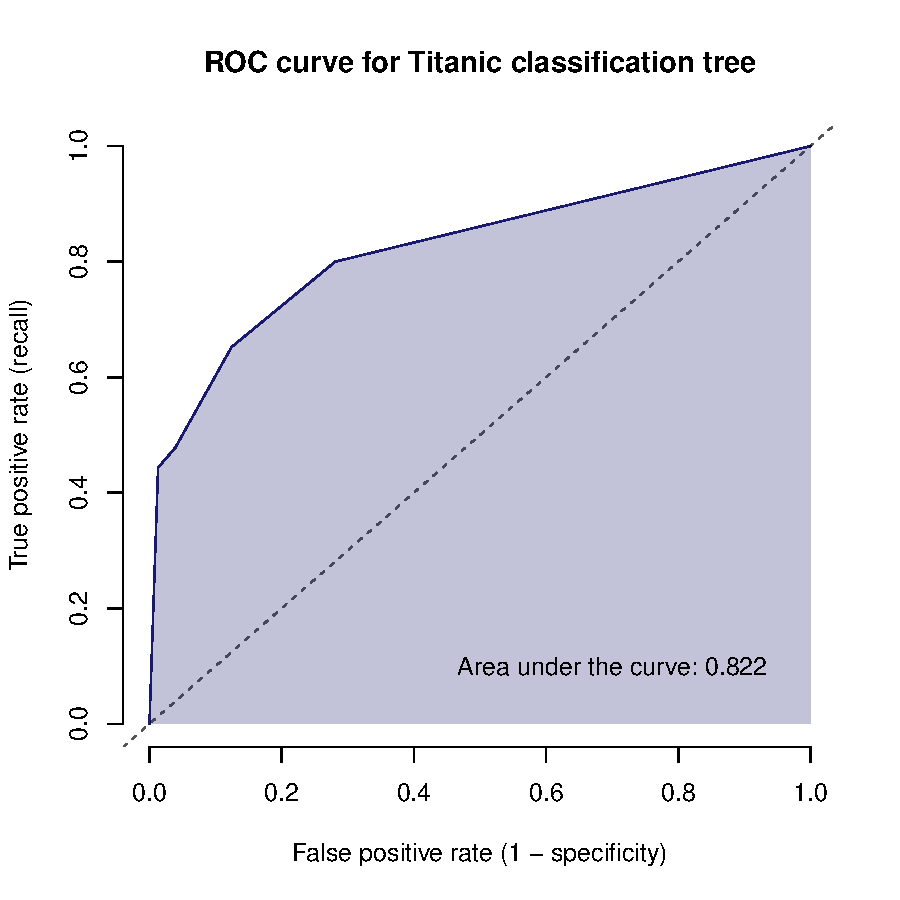
\includegraphics[height=\textheight]{pics/Titanic_tree_roc_shaded}
\end{frame}

\begin{frame}
	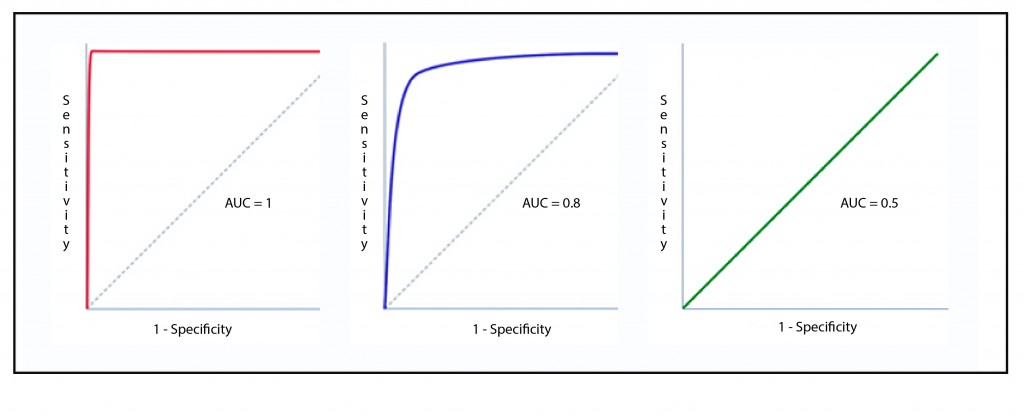
\includegraphics[width=\textwidth]{pics/ROC_curves-1024x417}
\end{frame}

\begin{frame}
	\begin{itemize}
		\item Besides the quality of a single-shot \textbf{predicted class}
		(``yes/no'', ``survive/die'', ...),
		\item we could also be interested in the \textbf{predicted
			probability}.
		\item E.g.: risk scores in medicine, betting, ...
	\end{itemize}
\end{frame}
\begin{frame}
	\begin{definition}
		A \textbf{probability} is a number $p$ such that the proportion of events
		given that number is about $p$.
	\end{definition}
	
	\begin{itemize}
		\item \textbf{Ideally}, the classification procedure (e.g. classification tree) outputs a predicted probability directly.
		\item \textbf{Unfortunately},
		\begin{itemize}
			\item Not all classifiers output something like a predicted
			probability (e.g. SVM);
			\item For many classifiers that do give a number between 0 and 1
			called a ``predicted probability'', \emph{the predicted
				probability does not give the correct proportion of events}.
		\end{itemize}
		\item This is called the ``\textbf{calibration} problem''.
	\end{itemize}
\end{frame}

\begin{frame}{Calibration plot}
	\begin{definition}
		A \textbf{probability} is a number $p$ such that the proportion of events
		given that number is about $p$.
	\end{definition}
	
	\begin{itemize}
		\item A predicted probability is calibrated when it conforms to the
		definition above;
		\item Check this using a \textbf{calibration plot}.
	\end{itemize}
\end{frame}
\begin{frame}
	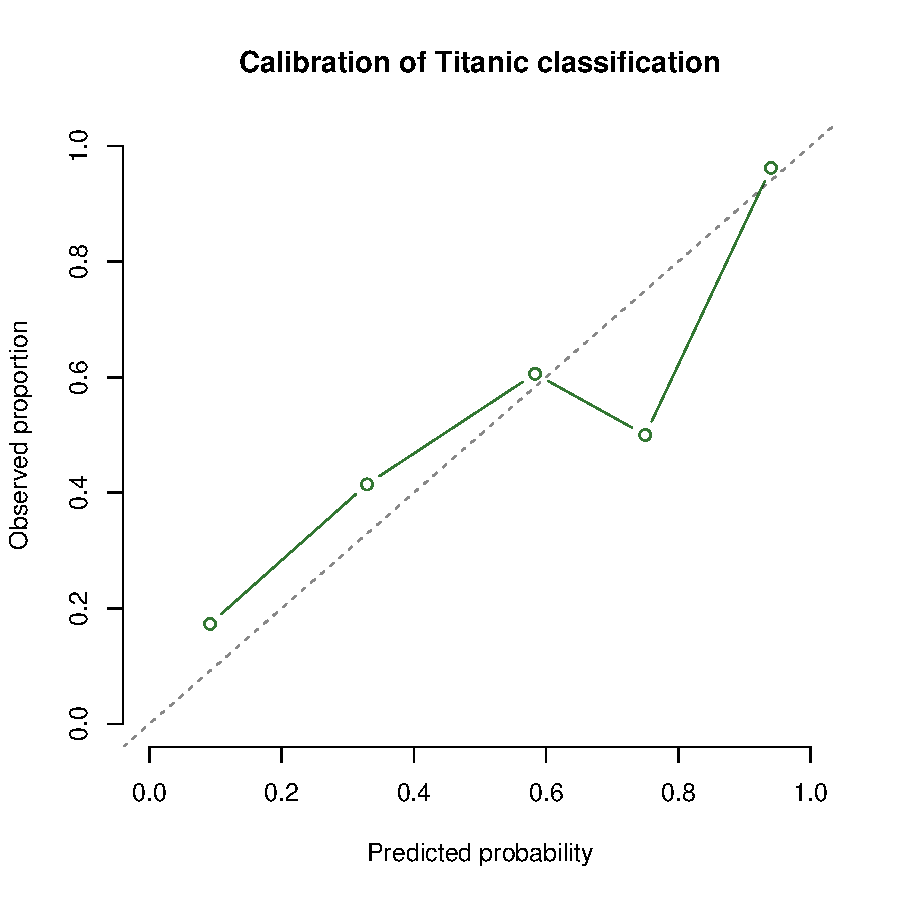
\includegraphics[height=\textheight]{pics/Titanic_tree_calibration}
\end{frame}

\begin{frame}{Post-hoc probability calibration}
	\begin{itemize}
		\item Some libraries allow you to tweak the predicted probabilities
		so they fit on the curve. This is called ``probability
		calibration''.
		\item There are many methods, but the most commonly used one takes a
		classification model we know is calibrated (``logistic
		regression'') and applies it to the uncalibrated scores outputted
		by the classifier;
		\item You may encounter this in your readings.
	\end{itemize}
\end{frame}
\begin{frame}
	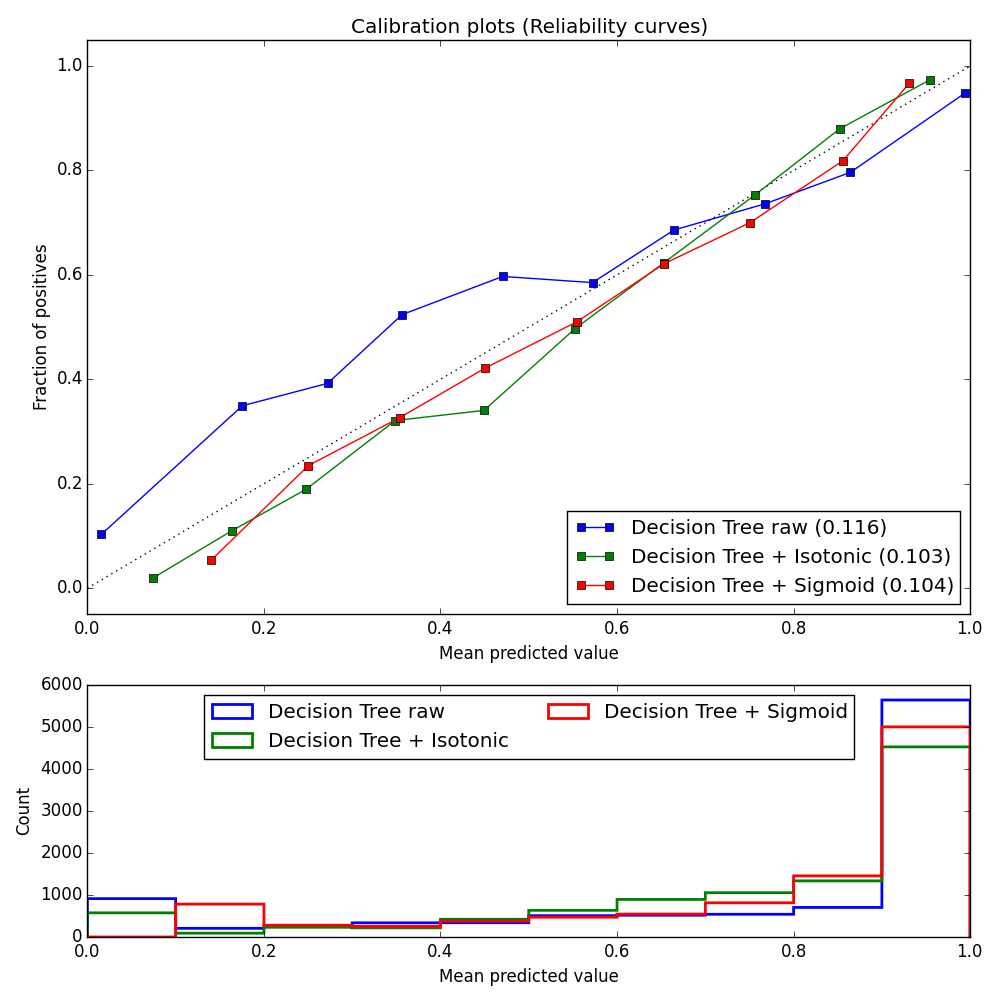
\includegraphics[height=\textheight]{pics/DT-calibration.png}
\end{frame}


\begin{frame}{MSE (``Brier score'')}
	\begin{itemize}
		\item By saying Yes = 1 and No = 0, we can also evaluate the Mean Square Error (MSE):
		$$
		\text{MSE} =    n^{-1} \sum_i (\hat{p}_i - y_i)^2
		$$
		\item Some call this the ``Brier score'' (only for classification!)
		\item Turns out MSE can be reworked  into two terms:
		
		\begin{equation*}
			\begin{split}
				\text{MSE} = \text{Calibration term}\; + \\\text{AUC term}
			\end{split}
		\end{equation*}
		\item[] {\color{gray} (Both terms are such that smaller is better)}
		\item In other words, the MSE conflates calibration and AUC;
		\item It is useful if you're interested in both.
	\end{itemize}
\end{frame}


\begin{frame}{  Class imbalance}
	\begin{itemize}
		\item In the \emph{Titanic} example, the outcome classes are pretty
		evenly balanced;
		\item That is not typical of many applications:
		\item[] debt default; illness; activity; buy/don't buy;
		tank/dog/selfie/..; solid/liquid/gas/plasma; ...
		\item When at least one class has very few observations, this is
		called \textbf{class imbalance}.
	\end{itemize}
\end{frame}

\begin{frame}{Class imbalance}
	\begin{itemize}
		\item Measures such as SEN/SPE/ACC/F1 emphasize larger classes;
		\item What if the smaller classes are the most interesting?
	\end{itemize}
	
	\medskip
	Some solutions:
	\begin{itemize}
		\item Show baseline / improvement over baseline
		\item Pick a better metric of interest
		\item Weigh your TP / FP / TN / FN in a specific way (e.g., based on cost?)
	\end{itemize}
	
\end{frame}


\section{Break}
\begin{frame}
	Break
\end{frame}

\section{Short recap: trees!}
\begin{frame}
	Short recap: Trees!
\end{frame}

\begin{frame}{Prediction tree: wood you survive the \emph{Titanic}?}
	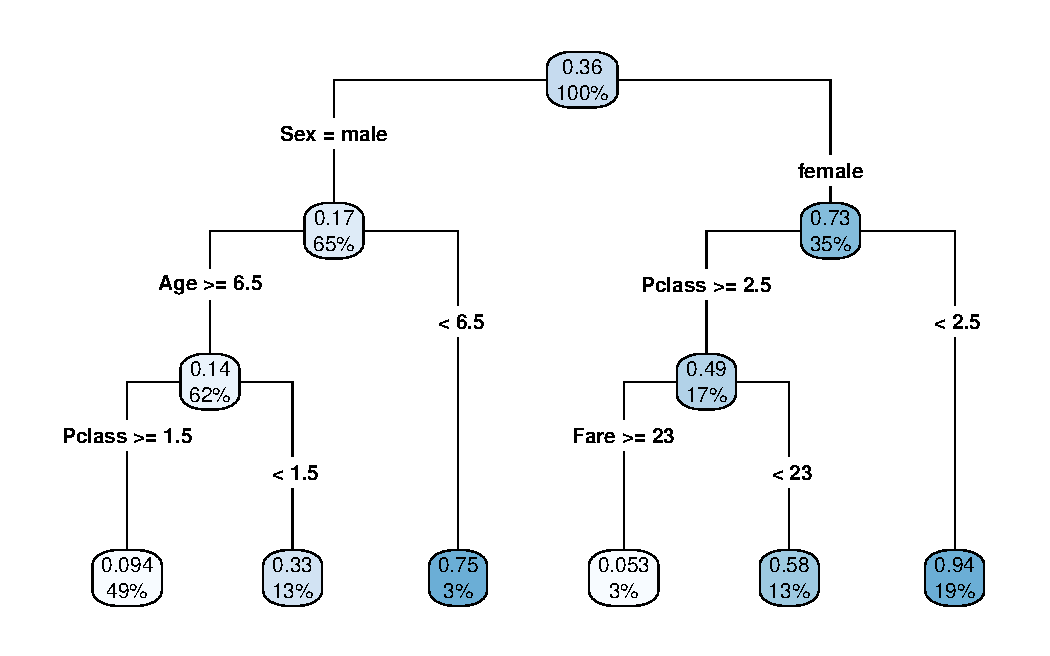
\includegraphics[width=0.78\textwidth]{pics/Titanic_tree}
\end{frame}

\begin{frame}{Recursive partitioning}
	\begin{enumerate}
		\item Find the split that makes observations as similar as possible on the outcome within that split;
		\item Within each resulting group, do (1).
	\end{enumerate}
	
	\bigskip
	\begin{itemize}
		\item Criteria for ``as similar as possible'': Purity, Reduction in MSE, ...
		\item Early stopping: add after (2):
		\begin{itemize}
			\item ``unless there are fewer than $n_{\text{min}}$ observations in the group'' (typically 10);
			\item ``unless the total complexity of the model becomes more than $cp$'' (typically 0.05);
		\end{itemize}
	\end{itemize}
\end{frame}

\begin{frame}{Choosing complexity}
	\begin{enumerate}
		\item Use recursive binary splitting to grow a large tree on the
		training data, stopping only when each terminal node has
		fewer than some minimum number of observations.
		\item Apply cost complexity pruning to the large tree in order to
		obtain a sequence of best subtrees, as a function of $\alpha$.
		\item Use $K$-fold cross-validation to choose $\alpha$. For each
		$k = 1, \ldots, K$:
		\begin{enumerate}
			\item[3.1]  Repeat Steps 1 and 2 on the $(K−1)/K$th fraction of the training
			data, excluding the $k$th fold.
			\item[3.2] Evaluate the model accuracy on the data in
			the left-out $k$th fold, as a function of $\alpha$.
		\end{enumerate}
		\item[] Average the results, and pick $\alpha$ to minimize the average
		error.
		\item Return the subtree from Step 2 that corresponds to the
		chosen value of $\alpha$.
	\end{enumerate}
	
	\vfill
	{\emph{\color{gray}\footnotesize{Source: Hastie \& Tibshirani}}}
\end{frame}

\begin{frame}
	{Advantages and Disadvantages of Trees}
	\begin{itemize}
		\item[+] Trees are very easy to explain to people. (?)
		\item[+] Trees can be displayed graphically, and are easily (??)
		interpreted even by a non-expert
		\item[+] Trees can easily handle qualitative predictors without the
		need to create dummy variables.
		\item[-] Trees are low bias but high variance $\rightarrow$ generally do not have the same level of
		predictive accuracy as other approaches.
	\end{itemize}
	
	However, by \textbf{aggregating many decision trees}, the predictive
	performance of trees can be substantially improved.
	\vfill
	{\emph{\color{gray}\footnotesize{Source: Hastie \& Tibshirani}}}
\end{frame}
\section{Bagging}
\begin{frame}
	Bagging
\end{frame}

\begin{frame}
	{Bagging: the general idea}
	
	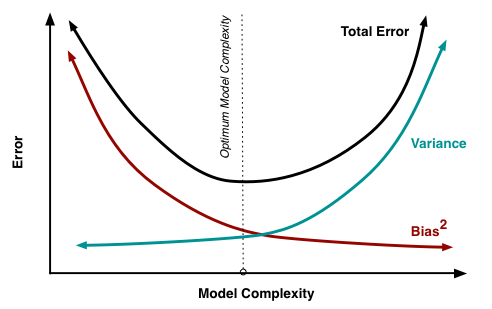
\includegraphics[width=.5\textwidth]{pics/biasvariance.png}
	
	\begin{itemize}
		\item $\downarrow$bias, $\uparrow$variance $\rightarrow$ Predictions differ strongly and meaninglessly across training sets
		\item[\textbf{IDEA}] Use different training sets to create different $\downarrow$B$\uparrow$V models, then \textbf{average the predictions}
	\end{itemize}
\end{frame}

\begin{frame}{Bootstrap aggregating (bagging)}
	
	\begin{itemize}
		\item Problem: we don't have different training sets (just one)
		\item Solution: ``bootstrapping''
		\item[] 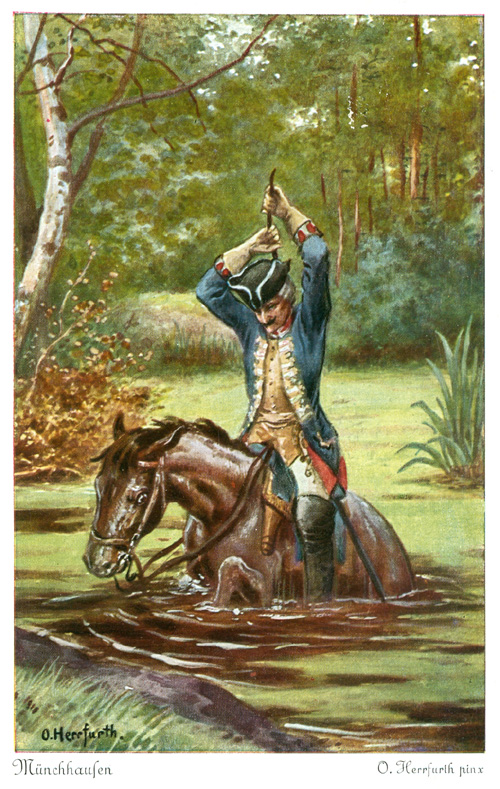
\includegraphics[height=0.5\textheight]{pics/munchausen.jpg}
	\end{itemize}

\end{frame}

\begin{frame}{Bootstrapping for aggregation}
	Do the following $B$ times:
	\begin{itemize}
		\item Resample $N$ values \textbf{with replacement} from training sample (with $N$ observations)
		\item Fit model (tree?) on each bootstrap sample
		\item On average, 2/3 of the training instances are selected
		\item The rest is "out-of-bag"
	\end{itemize}
\end{frame}

\begin{frame}
	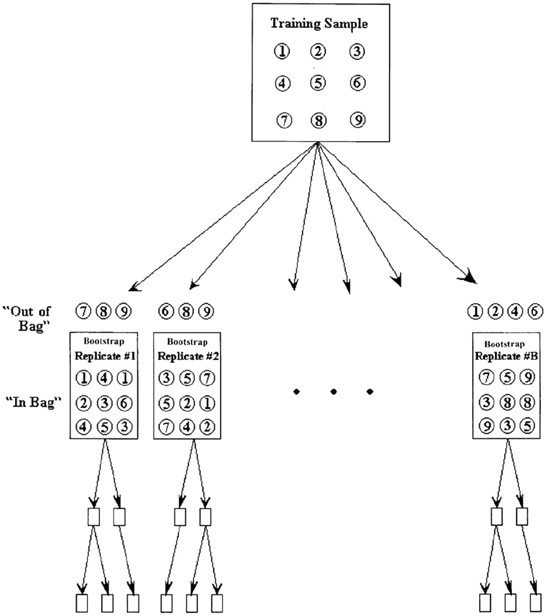
\includegraphics[height=0.95\textheight]{pics/bagging.png}
\end{frame}

\begin{frame}{Bootstrap ensemble}
	\begin{itemize}
		\item For new data, combine the predictions of the $B$ models
		\item Majority vote for classification; simple average for regression, 
		\item[]
		\item Useful bonus: Out-of-bag instances can serve as validation set for each model!
	\end{itemize}
\end{frame}

\begin{frame}{Bagged trees (``forest'')}
	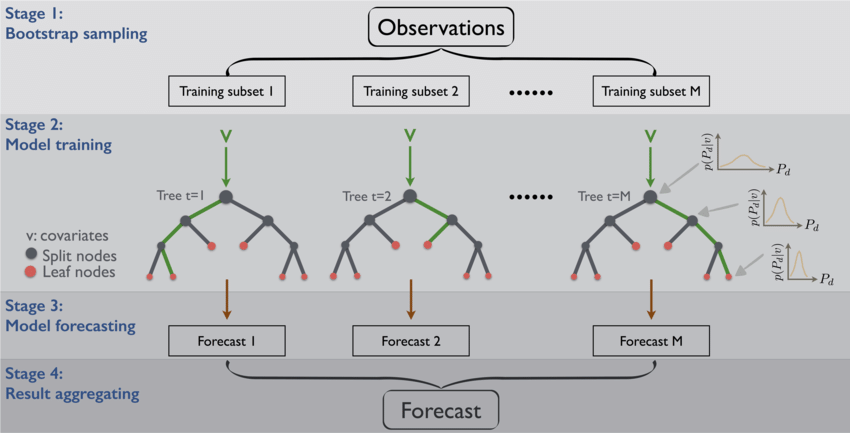
\includegraphics[width=0.9\textwidth]{pics/rf.png}
\end{frame}

\begin{frame}{Random forest}
	\begin{itemize}
		\item ``Wisdom of Crowds'': the collective knowledge of a diverse and independent body of people typically exceeds the knowledge of any single individual, and can be harnessed by voting. \referto{Hastie and Tibshirani, p. 286}
		\item Bagged trees are not diverse and independent: they are likely to choose similar splits at the higher levels
		\item A \textbf{random} forest is bootstrap aggregated trees with a handicap: at each split, consider only $m$ out of the $p$ predictors $\to$ \textit{decorrelating} the trees
	\end{itemize}	
\end{frame}

\begin{frame}{Random forest}
When $m = p$, standard bagging, but usually $m = \sqrt{p}$

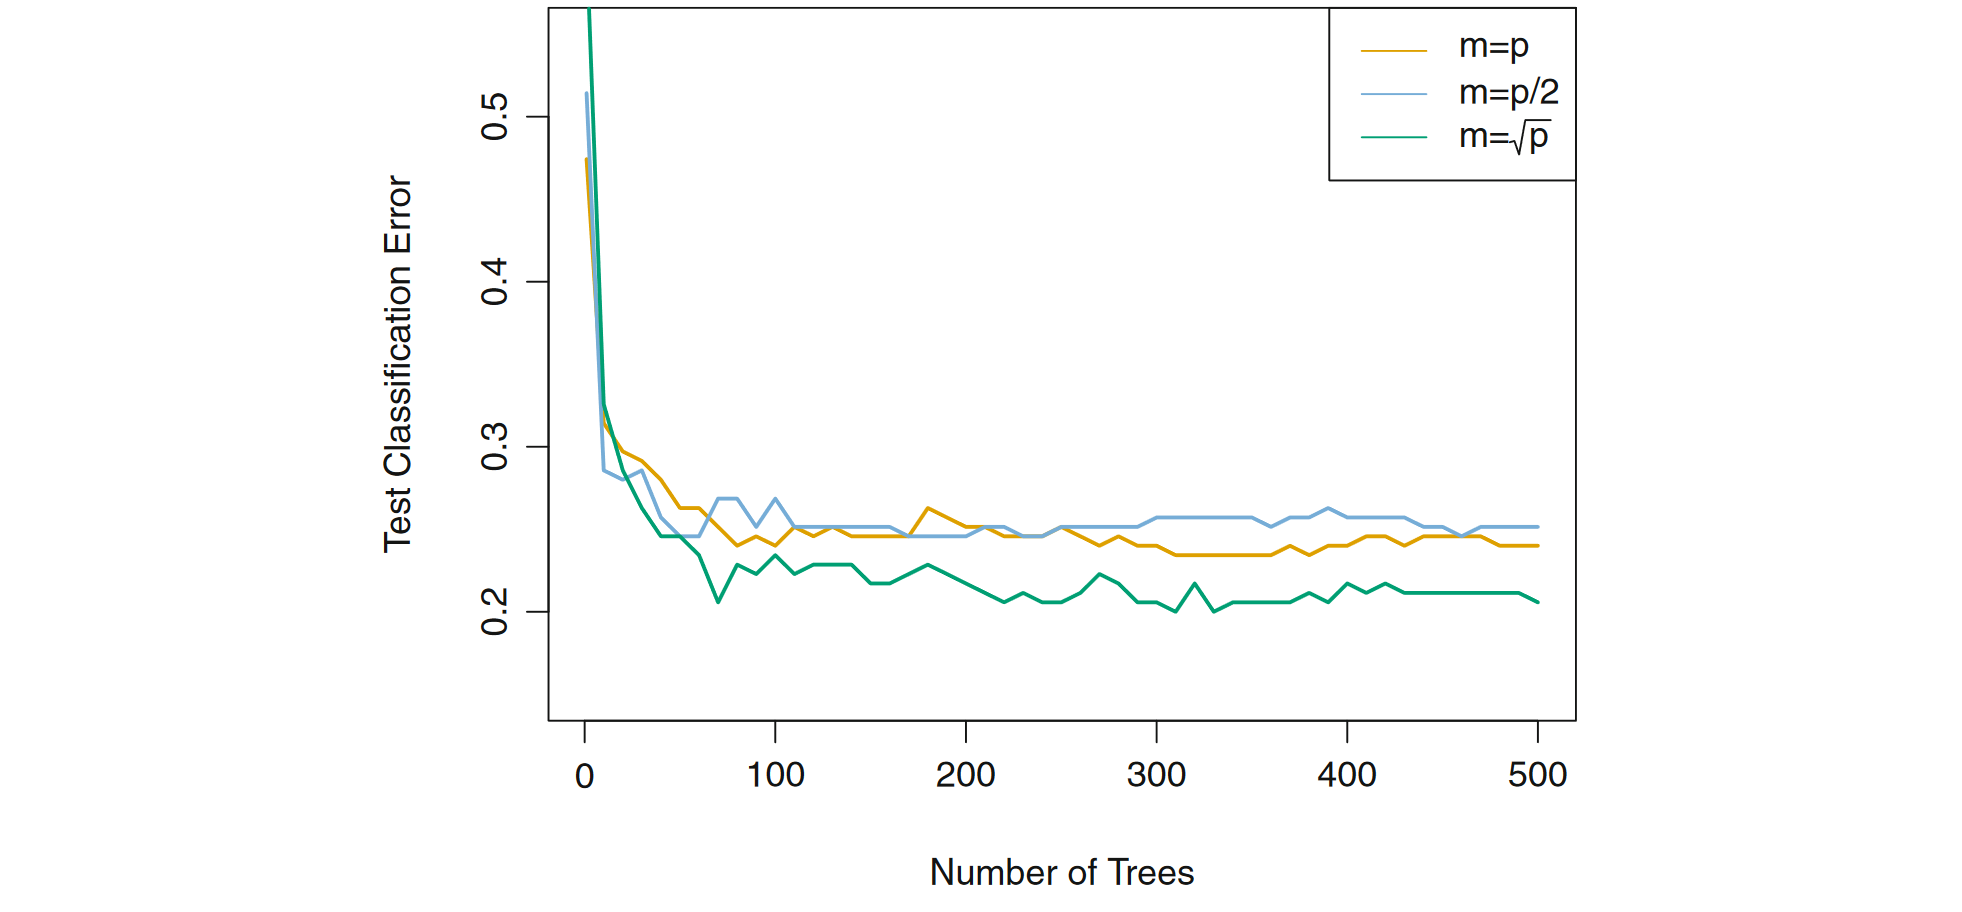
\includegraphics[width=0.8\textwidth]{pics/rf_mp.png}
\referto{ISLR, figure 8.10}
	
\end{frame}

\section{Boosting}
\begin{frame}
	Boosting
\end{frame}

\begin{frame}
	{Boosting: the general idea}
	
	\begin{itemize}
		\item $\uparrow$bias, $\downarrow$variance $\rightarrow$ Predictions stable, but wrong for some proportion of the training data
		\item[\textbf{IDEA}] Fit $\uparrow$B$\downarrow$V models consecutively, to parts where the previous models don't fit well
		\item Learn from mistakes of the previous models
		\item Average the predictions for new data: combine ``weak'' classifiers into powerful ``committee''
	\end{itemize}  
\end{frame}

\begin{frame}{Boosting with decision stumps}
 Weak learner: decision tree with 1 split (``decision stump'')\\

	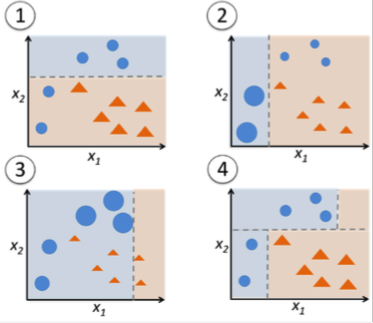
\includegraphics[width=0.35\textwidth]{pics/boosting.png}
	\vfill
	\referto{https://sebastianraschka.com/faq/docs/bagging-boosting-rf.html}
\end{frame}

\begin{frame}{Boosting with decision stumps}
	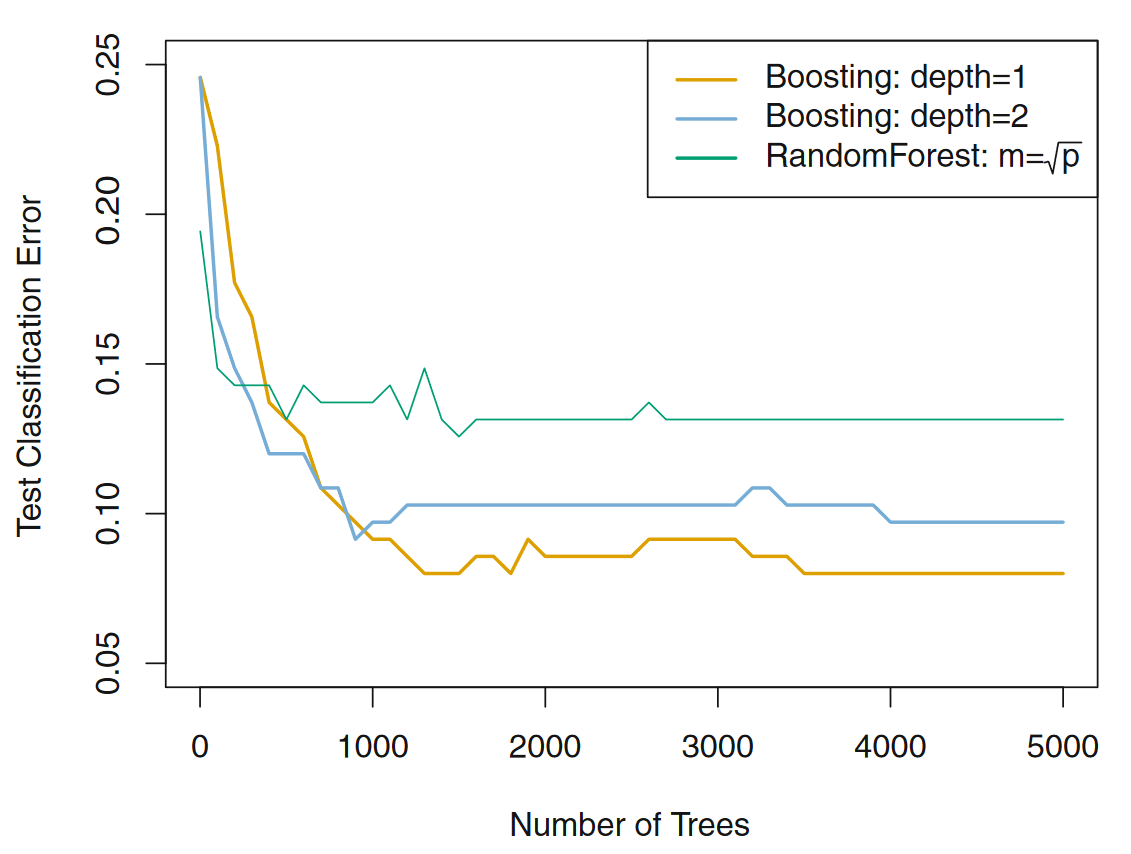
\includegraphics[width=0.5\textwidth]{pics/boosting_result.png}
	
	\referto{ISLR, figure 8.11}
\end{frame}


\section{Conclusion}

\begin{frame}{Conclusion}
	\begin{itemize}
		\item There are different classification performance metrics, suitable for different situations
		\item Class imbalance may affect the interpretation of classification performance
		\item ROC curve can be made for probabilistic classifiers
		\item Predicted probabilities can be calibrated
		\item[]
		\item Ensemble methods combine sets of base models (e.g., trees);
		\item Prediction from ensemble is average or majority vote;
		\item Bagging: ensemble (from bootstraps) of $\uparrow$V$\downarrow$B models;
		\item Boosting: ensemble (from high residuals) of $\uparrow$B$\downarrow$V models.
		\item Ensembles are very useful: often work well out of the box, state-of-the-art in many competitions
	\end{itemize}
\end{frame}
\begin{frame}
	
\begin{center}
	\emph{Have a nice day!}    
\end{center}
	
\end{frame}
\end{document}

